\chapter{量子估计、Rayleigh 极限与 SPADE 亚分辨}
\label{chap:e12}

\begin{chapteropening}
一百多年来，天文学家判断"两颗星能不能分开"，靠的都是同一句话：两个衍射斑的主峰要隔开得够远，中间要能看出一道凹槽。这就是 Rayleigh 判据。可是请想一想——如果我事先就\emph{知道}天上是两颗等亮的星，只是不知道它们隔多远，那么"看不出凹槽"真的等于"测不出间距"吗？这一章要把"分辨率"这件事彻底翻新：不再问"像面上能不能分成两个峰"，而问"给定这么多光子、这么一个点扩散函数，我把两颗星的角间距估计到多准"。换句话说，我们把成像判据升级成一个\textbf{估计问题}（estimation problem）。一旦这样问，就会冒出一个惊人的事实：当两颗星靠得很近时，普通成像会以 \(s^2\) 的速度把间距信息丢光（这就是所谓的 Rayleigh 诅咒），可那份信息其实\emph{根本没离开光场}——只是被"逐像素记录位置"这种笨办法漏掉了。换一种测量——先把光投到一组空间模式上再数光子，也就是 SPADE——就能把它捞回来。本章从高斯点扩散函数出发，一步不跳地推出这一切，最后把同一套 Fisher 信息语言搬到公里级长基线的强度干涉上，看看两条工程路线各自的软肋在哪里。
\end{chapteropening}


\section{从"能不能分成两个峰"到"能把间距估到多准"}
\label{sec:e12-rayleigh}

先把最熟悉的那条线画出来。一台口径 \(D\)、工作在波长 \(\lambda\) 的望远镜，对一个点源成像，得到的不是一个点，而是一小片衍射斑（圆孔的情形是 Airy 斑）。两个点源要"分开"，经典的 Rayleigh 判据说：一个源衍射斑的主峰，要正好落在另一个源衍射斑的第一个暗环上。对圆孔，这个角间距是

\begin{equation}
  \theta_{\rm R}=1.22\,\frac{\lambda}{D}.
  \label{eq:e12-rayleigh}
\end{equation}
\begin{formulaexplain}
\(\theta_{\rm R}\)：Rayleigh 角尺度（弧度）。\(\lambda\)：观测波长（米）。\(D\)：望远镜口径（米）。系数 \(1.22\) 来自圆孔 Airy 斑第一个暗环的位置。它是一条\emph{成像}判据，不是估计的终极极限。
\end{formulaexplain}

逐符号说明并代个真实数字。\(\theta_{\rm R}\) 以弧度计；换成天文学惯用的毫角秒要乘 \(206265\times10^3\)（因为 \(1\,\mathrm{rad}=206265''=2.06\times10^{8}\,\mathrm{mas}\)）。一台 \(D=8\,\mathrm{m}\) 的望远镜，在 \(\lambda=500\,\mathrm{nm}=5\times10^{-7}\,\mathrm{m}\) 处，
\[
  \theta_{\rm R}=1.22\times\frac{5\times10^{-7}}{8}
  =7.6\times10^{-8}\,\mathrm{rad}
  \approx15.7\,\mathrm{mas}.
\]
换成 \(30\,\mathrm{m}\) 的巨镜，同一波长下约 \(4.2\,\mathrm{mas}\)。这些数字告诉我们衍射斑有多大——但它们\emph{没有}告诉我们"两颗只隔 1 毫角秒的星到底测不测得出"。要回答后一个问题，得换一套语言。

为了把代数看清楚，我们把二维圆孔换成一维高斯点扩散函数（point spread function，简称 PSF）。这不是偷懒：高斯 PSF 保留了"有限宽度的响应核"这个核心，又让每一步积分都能手算出来。记

\begin{equation}
  h(x)=\frac{1}{\sqrt{2\pi}\,\sigma}\,
       \exp\!\left(-\frac{x^{2}}{2\sigma^{2}}\right).
  \label{eq:e12-gaussian-psf}
\end{equation}
\begin{formulaexplain}
\(h(x)\)：归一化点扩散函数（单位是长度或角度的倒数，积分为 1）。\(x\)：像面坐标或等效角坐标。\(\sigma\)：PSF 宽度，扮演衍射斑半径的角色，量级约 \(0.4\lambda/D\) 到 \(0.5\lambda/D\)。
\end{formulaexplain}

这里 \(x\) 若用角坐标，\(\sigma\) 也就是角宽度 \(\sigma_\theta\)，量级约 \(0.5\lambda/D\)——对上面那台 8 米镜，\(\lambda/D=6.25\times10^{-8}\,\mathrm{rad}\approx12.9\,\mathrm{mas}\)，故 \(\sigma_\theta\approx0.5\times12.9\approx6\,\mathrm{mas}\)。它就是"衍射斑有多胖"的一个数。

现在放两颗\textbf{等亮、互不相干}（equal-brightness, mutually incoherent）的点源，把它们的质心放在原点，一颗在 \(+s/2\)、一颗在 \(-s/2\)，角间距就是 \(s\)。"互不相干"很关键：它意味着我们要把两颗星各自的\emph{强度}相加，而不是把振幅相加再平方（第 \ref{chap:e10} 章讲空间相干时反复强调过这条界线）。于是探测到的单个光子落在像面位置 \(x\) 的概率密度是两个平移 PSF 的等权平均：

\begin{equation}
  p(x\mid s)=\tfrac12\,h\!\left(x-\tfrac{s}{2}\right)
            +\tfrac12\,h\!\left(x+\tfrac{s}{2}\right).
  \label{eq:e12-direct-prob}
\end{equation}
\begin{formulaexplain}
\(p(x\mid s)\)：给定间距 \(s\) 时，一个光子落在 \(x\) 的概率密度。两个 \(h\) 分别来自质心两侧的星，系数 \(\tfrac12\) 表示等亮。直接成像看到的，就是这两个衍射斑的强度叠加。
\end{formulaexplain}

\paragraph{关键一步：小间距先表现为"变胖"，不是"分家"}
\label{sec:e12-taylor}

现在做本章第一处、也是最能颠覆直觉的推导。我们要看：当 \(s\ll\sigma\) 时，\(p(x\mid s)\) 到底怎么随 \(s\) 变。用到的工具是\textbf{泰勒展开}（Taylor expansion）——把一个平移了一点点的函数，用它在原处的值和各阶导数展开。对平移量 \(\pm s/2\)，展到二阶：

\[
  h\!\left(x\pm\tfrac{s}{2}\right)
  =h(x)\;\pm\;\frac{s}{2}\,h'(x)
   \;+\;\frac{1}{2}\left(\frac{s}{2}\right)^{2}h''(x)
   \;+\;\mathcal{O}(s^{3})
  =h(x)\pm\frac{s}{2}h'(x)+\frac{s^{2}}{8}h''(x)+\mathcal{O}(s^{3}).
\]

把这两条代回式 \eqref{eq:e12-direct-prob}。注意 \(\tfrac12\) 的权重，以及\textbf{一阶项符号相反}：一颗星往右挪、一颗往左挪，正负 \(h'(x)\) 恰好抵消。于是

\[
  p(x\mid s)
  =\tfrac12\Big[h+\tfrac{s}{2}h'+\tfrac{s^{2}}{8}h''\Big]
  +\tfrac12\Big[h-\tfrac{s}{2}h'+\tfrac{s^{2}}{8}h''\Big]
  +\mathcal{O}(s^{4})
  =h(x)+\frac{s^{2}}{8}\,h''(x)+\mathcal{O}(s^{4}).
\]

停下来品一品这个结果。\emph{间距 \(s\) 进入像面的最低阶是 \(s^2\)，而且是通过二阶导数 \(h''\)}。二阶导数在高斯峰顶是负的、在两翼是正的，效果就是"把峰压低一点、把肩膀抬高一点"——也就是让衍射斑\textbf{变胖}。所以两颗近星在像面上第一件干的事不是"分成两个峰"，而是"整体变宽一点点"。"看不出两个峰"因此\emph{根本不等于}"没有信息"；信息藏在一个二阶小量里，只是普通成像很难把它从噪声里刨出来。

这就自然引向下一节的问题：这份藏在二阶展宽里的信息，到底值多少？要量化它，需要 Fisher 信息。


\section{Fisher 信息与 Cramér--Rao 下界：数据里到底有多少信息}
\label{sec:e12-fisher}

假设一次观测最终留下 \(N_\gamma\) 个可用于估计的源光子（扣掉背景、坏像素、选择效应之后）。每个光子的位置 \(x_i\) 都是从分布 \(p(x\mid s)\) 里独立抽出来的样本。我们手上握着一批 \(\{x_i\}\)，想反推出 \(s\)。统计学给这类问题一把标尺：似然函数（likelihood）。它是"如果真实间距是 \(s\)，我观测到这批光子的概率有多大"。取对数把连乘变连加：

\begin{equation}
  \ln\mathcal{L}(s)=\sum_{i=1}^{N_\gamma}\ln p(x_i\mid s).
  \label{eq:e12-loglike}
\end{equation}
\begin{formulaexplain}
\(\ln\mathcal{L}(s)\)：对数似然。\(x_i\)：第 \(i\) 个光子的位置。\(N_\gamma\)：有效源光子数。它把每个光子对"间距等于 \(s\)"这个假设的支持累加起来。
\end{formulaexplain}

似然作为 \(s\) 的函数越尖，就越能把 \(s\) 钉死。"有多尖"由\textbf{Fisher 信息}（Fisher information）量化——它是对数似然对参数的斜率的平方的期望，等价地也可写成概率密度对参数的敏感度。对单参数 \(s\)，且 \(N_\gamma\) 个光子独立同分布，

\begin{equation}
  F_{ss}=N_\gamma\int
  \frac{1}{p(x\mid s)}
  \left[\frac{\partial p(x\mid s)}{\partial s}\right]^{2}\mathrm{d}x.
  \label{eq:e12-fisher-def}
\end{equation}
\begin{formulaexplain}
\(F_{ss}\)：间距 \(s\) 的总 Fisher 信息（单位：角度的 \(-2\) 次方）。\(\partial p/\partial s\)：间距变一点点、概率密度变多快。\(1/p\)：给每个位置按其发生概率赋统计权重。\(N_\gamma\)：光子越多、信息越多。
\end{formulaexplain}

Fisher 信息之所以重要，是因为它给任何\emph{无偏}估计量 \(\hat s\)（无偏：平均而言不系统偏高或偏低）设了一条误差地板，叫 \textbf{Cramér--Rao 下界}（Cramér--Rao bound）：

\begin{equation}
  \mathrm{Var}(\hat s)\ \ge\ \frac{1}{F_{ss}}.
  \label{eq:e12-crb}
\end{equation}
\begin{formulaexplain}
\(\mathrm{Var}(\hat s)\)：估计量 \(\hat s\) 的方差。式子说：Fisher 信息越大，任何无偏估计能达到的最小统计误差越小。取平方根得 \(\Delta s\ge 1/\sqrt{F_{ss}}\)。
\end{formulaexplain}

这条不等式是本章的度量衡：以后不管谁声称"能测出 0.1 毫角秒的间距"，都得回到 \(1/\sqrt{F_{ss}}\) 看看数据里到底够不够信息。

\paragraph{直接成像的 Rayleigh 诅咒：\texorpdfstring{$F_{ss}\propto s^{2}$}{Fss 正比于 s 平方}}
\label{sec:e12-curse}

现在把上一节的展开结果代进 \eqref{eq:e12-fisher-def}，算出直接成像对间距的 Fisher 信息。我们已经有
\[
  p(x\mid s)=h(x)+\frac{s^{2}}{8}h''(x)+\mathcal{O}(s^{4}),
  \qquad
  \frac{\partial p}{\partial s}=\frac{s}{4}\,h''(x)+\mathcal{O}(s^{3}).
\]
（第二式就是对第一式逐项求 \(s\) 的导数：\(\partial_s(s^2/8)=s/4\)。）于是被积函数在小 \(s\) 下
\[
  \frac{1}{p}\left(\frac{\partial p}{\partial s}\right)^{2}
  \approx\frac{1}{h(x)}\cdot\frac{s^{2}}{16}\big[h''(x)\big]^{2}
  =\frac{s^{2}}{16}\,\frac{[h''(x)]^{2}}{h(x)},
\]
其中分母里的 \(p\approx h\)（因为修正项是 \(s^2\) 的高阶小量）。剩下要算一个积分 \(\int [h'']^2/h\,\mathrm{d}x\)。这一步要用到\textbf{高斯矩}（Gaussian moments）：对方差为 \(\sigma^2\) 的高斯分布 \(h\)，有 \(\langle x^2\rangle=\sigma^2\)、\(\langle x^4\rangle=3\sigma^4\)（三是标准的高斯四阶矩因子）。先算 \(h''\)。由 \eqref{eq:e12-gaussian-psf}，
\[
  h'(x)=-\frac{x}{\sigma^{2}}h(x),\qquad
  h''(x)=\frac{x^{2}-\sigma^{2}}{\sigma^{4}}\,h(x).
\]
（第二式：对 \(h'=-(x/\sigma^2)h\) 再求导，用乘积法则 \(h''=-\tfrac1{\sigma^2}h-\tfrac{x}{\sigma^2}h'=-\tfrac1{\sigma^2}h+\tfrac{x^2}{\sigma^4}h\)。）代入积分：
\[
  \int\frac{[h'']^{2}}{h}\,\mathrm{d}x
  =\int\frac{(x^{2}-\sigma^{2})^{2}}{\sigma^{8}}\,h(x)\,\mathrm{d}x
  =\frac{1}{\sigma^{8}}\big\langle(x^{2}-\sigma^{2})^{2}\big\rangle.
\]
把括号展开，用两个已知矩：
\[
  \big\langle(x^{2}-\sigma^{2})^{2}\big\rangle
  =\langle x^{4}\rangle-2\sigma^{2}\langle x^{2}\rangle+\sigma^{4}
  =3\sigma^{4}-2\sigma^{4}+\sigma^{4}=2\sigma^{4}.
\]
所以 \(\int[h'']^2/h\,\mathrm{d}x=2\sigma^4/\sigma^8=2/\sigma^4\)。合起来，单个光子的 Fisher 信息是 \(\tfrac{s^2}{16}\cdot\tfrac{2}{\sigma^4}=\tfrac{s^2}{8\sigma^4}\)，乘以 \(N_\gamma\)：

\begin{equation}
  F_{ss}^{\rm direct}\simeq N_\gamma\,\frac{s^{2}}{8\sigma^{4}},
  \qquad s\ll\sigma.
  \label{eq:e12-direct-fisher}
\end{equation}
\begin{formulaexplain}
\(F_{ss}^{\rm direct}\)：直接成像对间距的 Fisher 信息。要命的是它\emph{正比于 \(s^{2}\)}：两颗星越靠近，像素数据对间距越不敏感，信息以平方速度掉向零。
\end{formulaexplain}

这就是\textbf{Rayleigh 诅咒}（Rayleigh curse）：把 \eqref{eq:e12-direct-fisher} 代进 Cramér--Rao 下界 \eqref{eq:e12-crb}，误差地板 \(\Delta s\ge \sqrt{8}\,\sigma^2/(s\sqrt{N_\gamma})\) 随 \(s\to0\) 发散——间距越小，要达到同样精度所需的光子数以 \(1/s^2\) 暴涨 \citep{2016PhRvX...6c1033T,2018Optic...5.1177P}。写成无量纲形式 \(q=s/\sigma\)，则单光子 \(F_{qq}^{\rm direct}\simeq q^2/8\)，纯数字地告诉你"分辨尺度以下，直接成像几乎瞎了"。图 \ref{fig:e12-rayleigh} 把这条二次下降的蓝线画了出来。

\begin{figure}[tbp]
\centering
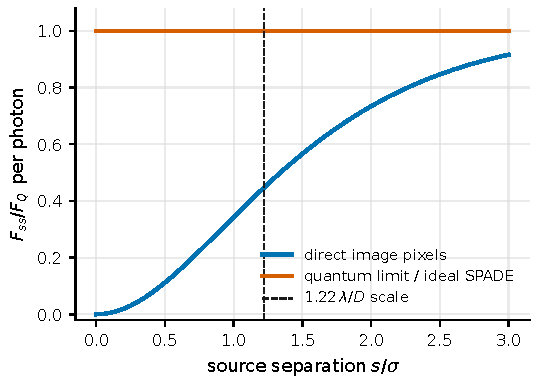
\includegraphics[width=0.82\linewidth]{figures/generated/chapter_08/ch08_rayleigh_information.pdf}
\caption{两颗等亮不相干高斯点源的间距信息。蓝线是由像面概率密度 \(p(x\mid s)\) 数值积分得到的直接成像 Fisher 信息（按量子极限归一化）；小间距时它以 \(s^2\) 掉向零，这就是 Rayleigh 诅咒。橙线是下一节的量子极限，即使 \(s\to0\) 也保持有限。竖虚线标出常用的 Rayleigh 角尺度。}
\label{fig:e12-rayleigh}
\end{figure}

\paragraph{检测问题不是估计问题}
\label{sec:e12-detection}

这里要划一条容易被忽略的界。上面整套 Fisher 语言默认我们\emph{已经接受}"天上是两颗等亮星"这个模型，只是不知道 \(s\)。这叫估计问题。另一类问题是"这到底是一颗星还是两颗星"——这叫\textbf{检测/模型选择}（detection / model selection）问题。两者不能混：检测问题里模型维数会变，而且 \(s=0\) 恰好落在参数空间的\emph{边界}上，常规的似然比近似（假设参数在内点、误差近高斯）在边界上未必成立，得靠模拟校准或贝叶斯证据来判。本章后面讲的所有"亚分辨增益"，都是在\emph{已接受双源模型}的前提下，把已经存在于光里的间距信息读得更干净——不是变魔术凭空造出一个源。

\paragraph{多参数：质心、亮度比、PSF 宽都会来抢信息}
\label{sec:e12-matrix}

真实观测里，间距 \(s\) 从来不是唯一未知量。质心位置 \(x_0\)、两颗星的亮度比 \(r\)、PSF 宽度 \(\sigma\)、背景 \(b\)……都得同时估。这时标量下界升级成\textbf{矩阵}版本。把所有参数排成向量 \(\bm\theta=(s,x_0,r,\sigma,b,\dots)\)，Fisher 信息成为一个矩阵：

\begin{equation}
  \mathrm{Cov}(\hat{\bm\theta})\ \succeq\ F^{-1},
  \qquad
  F_{\alpha\beta}=N_\gamma\int
  \frac{1}{p(x\mid\bm\theta)}
  \frac{\partial p}{\partial\theta_\alpha}
  \frac{\partial p}{\partial\theta_\beta}\,\mathrm{d}x.
  \label{eq:e12-fisher-matrix}
\end{equation}
\begin{formulaexplain}
\(F_{\alpha\beta}\)：Fisher 矩阵的第 \((\alpha,\beta)\) 元，比较参数 \(\theta_\alpha\)、\(\theta_\beta\) 对同一数据分布的影响。\(\mathrm{Cov}(\hat{\bm\theta})\succeq F^{-1}\)：协方差矩阵不小于 Fisher 矩阵的逆（矩阵不等式）。逆矩阵的对角元才是各参数的实际方差。
\end{formulaexplain}

关键在\emph{取逆}这一步。\(F\) 的非对角元记录参数间的\textbf{退化}（degeneracy）：如果两个参数对数据的影响"长得像"，它们的信息会互相纠缠，取逆后把误差放大。具体到亚分辨：未知质心会和间距混（把整幅图挪一点，很像把两颗星错开一点）；未知亮度比会在奇模式和偶模式之间重新分配信息；未知 PSF 宽度最阴险——它和双星间距都表现为"衍射斑变胖"（回想 \(s^2 h''\) 那一项！），两者几乎共线，若 \(\sigma\) 没被独立标定死，双星信号会被当成 PSF 变宽吸收掉。所以现实里报误差，不能只甩一个 \(1/\sqrt{F_{ss}}\)，得给出完整协方差、外加 PSF 标定误差、背景误差和模型误差。


\section{量子 Fisher 信息：把"测量方式"也放进优化}
\label{sec:e12-qfi}

到这里，一个尖锐的问题浮出来：直接成像的信息掉向零，那是\emph{光本身}就没带够信息，还是\emph{我们的测量方式}太笨？经典 Fisher 信息 \eqref{eq:e12-fisher-def} 是"先把测量方式定死（逐像素数光子），再问数据里有多少信息"。它把测量当成给定的。可量子力学允许的测量远不止"逐像素"一种——任意的正交投影、任意的干涉与模式分解都算数。

于是引入\textbf{量子 Fisher 信息}（quantum Fisher information，QFI）：在\emph{所有}量子力学允许的测量里取最优，同一束光原则上最多能读出多少参数信息。它是一切经典 Fisher 信息的上确界，\(F_{ss}\le F_{ss}^{Q}\)。QFI 只和光场的量子态怎么随参数变有关，和你选哪种探测器无关。

要写下这束光的态，我们借第 \ref{chap:e06} 章的弱热光结论。天体热光在每个相干时间模式里的平均光子数 \(\epsilon\ll1\)，所以密度矩阵近似是"真空 + 一点点单光子"：\(\rho\approx(1-\epsilon)|0\rangle\langle0|+\epsilon\,\rho_1\)。真空那一大块不点击、不带角信息——没有光子落下来，你无从知道两颗星隔多远。真正携带间距信息的，是那少数被探测到的\emph{单光子空间模式}。两颗等亮不相干点源的单光子部分是两个模式的等权混合：

\begin{equation}
  \rho_{1}(s)=\tfrac12\,\big|\psi_{+s/2}\big\rangle\big\langle\psi_{+s/2}\big|
             +\tfrac12\,\big|\psi_{-s/2}\big\rangle\big\langle\psi_{-s/2}\big|,
  \label{eq:e12-one-photon}
\end{equation}
\begin{formulaexplain}
\(\rho_1(s)\)：探测到一个光子时的空间模式密度矩阵。\(|\psi_{\pm s/2}\rangle\)：两颗星的光经过望远镜后，各自在像面形成的振幅模式（其模方就是平移了的 PSF）。不相干等亮 = 两个单光子态的等权概率混合。
\end{formulaexplain}

这里 \(|\psi_{\pm s/2}\rangle\) 是振幅 PSF，对高斯情形 \(\psi(x)\propto\exp[-x^2/(4\sigma^2)]\)（取模方 \(|\psi|^2\propto\exp[-x^2/(2\sigma^2)]=h\)，方差正好 \(\sigma^2\)）。

在正式抛结果之前，先让读者自己把那个关键的数落地。QFI 的大小，归根到底由振幅模式\emph{有多容易被平移区分}决定，而这由它的"动量方差"\(\Delta k^2=\int(\psi')^2\,\mathrm{d}x\) 定标——这一步用高斯就能手算。把归一化的 \(\psi(x)=(2\pi\sigma^2)^{-1/4}\exp[-x^2/(4\sigma^2)]\) 求导，\(\psi'(x)=-\dfrac{x}{2\sigma^2}\psi(x)\)，于是
\[
  \Delta k^2=\int\big[\psi'(x)\big]^2\,\mathrm{d}x
  =\frac{1}{4\sigma^4}\int x^2\,|\psi(x)|^2\,\mathrm{d}x
  =\frac{1}{4\sigma^4}\cdot\sigma^2
  =\frac{1}{4\sigma^2},
\]
用到了 \(\int|\psi|^2\,\mathrm{d}x=1\) 与 \(\int x^2|\psi|^2\,\mathrm{d}x=\sigma^2\)（同一条高斯二阶矩）。这个 \(1/(4\sigma^2)\) 正是下面单光子 QFI 里那个漂亮得出奇的数字的出处。在质心、亮度、PSF 宽都已知的理想条件下，对式 \eqref{eq:e12-one-photon} 那个 rank-2 混合态严格算 QFI，结果恰好是每光子 \(\Delta k^2\)：

\begin{equation}
  F_{ss}^{Q}=N_\gamma\,\frac{1}{4\sigma^{2}}.
  \label{eq:e12-qfi}
\end{equation}
\begin{formulaexplain}
\(F_{ss}^{Q}\)：所有允许测量能达到的间距信息\emph{上限}。\(\sigma\)：振幅模式对应的像面宽度。要害在于它\emph{不含 \(s\)}——\(s\to0\) 时它不消失，说明间距信息一直好端端待在光里，是直接成像把它漏掉了。
\end{formulaexplain}

需要对读者\emph{诚实}地交代一句：这里我们只算到了"定标尺度"\(\Delta k^2\)，而把 rank-2 混合态 QFI 的完整证明当作\textbf{已知结果引用}。它由 Helstrom 的量子估计理论奠基、经 Tsang 等人针对双源亚分辨给出显式值，我们在此直接采用 \citep{1969JSP.....1..231H,2016PhRvX...6c1033T}。混合态 QFI 要经由对称对数导数（symmetric logarithmic derivative，SLD）求解，严格推导超出本科范围，故不在此展开；但读者不必把 \eqref{eq:e12-qfi} 当"天上掉下来的"——\S\ref{sec:e12-spade} 会\emph{显式}造出 SPADE 这把尺，把经典 Fisher 信息一步步算到同一个 \(N_\gamma/(4\sigma^2)\)。这至少从下方确认了 \(F_{ss}^{Q}\ge N_\gamma/(4\sigma^2)\) 是可达的：既然存在一种真实测量能达到这个值，上限就不可能比它更低。

把 \eqref{eq:e12-qfi} 和直接成像的 \eqref{eq:e12-direct-fisher} 摆在一起看，反差刺眼：
\[
  \frac{F_{ss}^{\rm direct}}{F_{ss}^{Q}}
  =\frac{N_\gamma s^2/(8\sigma^4)}{N_\gamma/(4\sigma^2)}
  =\frac{s^2}{2\sigma^2}\ \xrightarrow{\,s\to0\,}\ 0.
\]
也就是说，在亚分辨区，直接成像用掉的信息占比以 \(s^2\) 趋零——绝大部分信息被白白丢掉了（图 \ref{fig:e12-rayleigh} 里蓝线掉下去、橙线不掉，画的就是这件事）。这不是望远镜绕过了衍射，而是"把测量方式也纳入优化"带来的裁决：信息在光里，就看你会不会读 \citep{1969JSP.....1..231H,2016PhRvX...6c1033T,2016OExpr..24.3684N}。下一节就造出那把"会读的尺"。


\section{SPADE：把小间距翻译成模式计数}
\label{sec:e12-spade}

QFI 只说"存在一种最优测量"，没说是哪一种。对高斯 PSF、等亮双源，那个最优（或接近最优）测量有个具体名字：\textbf{空间模式解调}（spatial-mode demultiplexing，SPADE）。它的想法一句话就能说清——\emph{别急着问光子落在哪个像素，先问它属于哪个正交空间模式，然后对每个模式分别数光子}。

对高斯 PSF，最自然的一组正交模式是 \textbf{Hermite--Gauss 模式}（Hermite--Gaussian modes），记作 \(u_0,u_1,u_2,\dots\)。它们其实是老熟人：第 \ref{chap:e04} 章的谐振子本征函数——一个高斯乘以 Hermite 多项式，\(u_0\) 是纯高斯、\(u_1\) 有一个节点、\(u_n\) 有 \(n\) 个节点。基模 \(u_0\) 恰好可以取成振幅 PSF 本身 \(\psi(x)\)。

\paragraph{为什么模式概率是 Poisson 分布}
\label{sec:e12-poisson}

现在算一颗星（位于 \(+s/2\)）的光落进各个模式的概率。它的振幅模式 \(\psi_{+s/2}(x)=\psi(x-s/2)\)，是把基模\emph{横向平移}了 \(d=s/2\)。这里可以借第 \ref{chap:e04} 章一个漂亮的对应：在谐振子语言里，把基态波函数在位置上平移一段 \(d\)，得到的正是一个\textbf{相干态}（coherent state）\(|\alpha\rangle\)，而相干态在数态（这里就是模式序号 \(n\)）上的占据概率是 Poisson 分布 \(|\langle n|\alpha\rangle|^2=e^{-|\alpha|^2}|\alpha|^{2n}/n!\)。位移 \(d\) 与 \(\alpha\) 的换算是 \(\alpha=d/(2x_{\rm zpf})\)，而对我们的模式，零点起伏尺度 \(x_{\rm zpf}=\sigma\)。所以

\[
  |\alpha|^{2}=\frac{d^{2}}{4\sigma^{2}}
  =\frac{(s/2)^{2}}{4\sigma^{2}}
  =\frac{s^{2}}{16\sigma^{2}}\ \equiv\ Q.
\]

另一颗星在 \(-s/2\)，位移是 \(-d\)，对应 \(\alpha\to-\alpha\)；但 Poisson 概率只依赖 \(|\alpha|^2\)，正负位移给出\emph{一模一样}的模式概率。于是两颗星的等权混合，其第 \(n\) 个模式的单光子点击概率就是

\begin{equation}
  p_{n}=e^{-Q}\,\frac{Q^{n}}{n!},
  \qquad
  Q=\frac{s^{2}}{16\sigma^{2}}.
  \label{eq:e12-spade-prob}
\end{equation}
\begin{formulaexplain}
\(p_n\)：光子落进第 \(n\) 个 Hermite--Gauss 模式的概率。\(Q\)：由间距和宽度拼出的无量纲"信号强度"，就是那个等效相干态的平均光子数。SPADE 把连续的间距，变成一列离散模式上的计数分布。
\end{formulaexplain}

这个 Poisson 形状用到了相干态的标准结果（第 \ref{chap:e06} 章）；如果你不想借谐振子，也可以直接算两个平移高斯与各 Hermite--Gauss 模式的重叠积分，会得到完全相同的 \(p_n\)。小 \(s\) 下展开：\(p_0=e^{-Q}\approx1-Q\)（几乎全部光子仍在基模），而
\[
  p_1=e^{-Q}Q\approx Q=\frac{s^{2}}{16\sigma^{2}},
\]
一小撮光漏进了第一阶（奇）模式 \(u_1\)。这一漏，正是间距信号本身。

\paragraph{第一阶模式的计数，与它为何能绕开诅咒}
\label{sec:e12-mode-fisher}

把概率乘以光子数，第一阶模式的期望计数是

\begin{equation}
  \langle n_1\rangle\simeq N_\gamma\,\frac{s^{2}}{16\sigma^{2}}.
  \label{eq:e12-n1}
\end{equation}
\begin{formulaexplain}
\(\langle n_1\rangle\)：第一阶模式里期望收到多少光子，等于总光子数乘以漏进该模式的概率 \(p_1\)。概率虽小，只要 \(N_\gamma\) 够大，就能攒成可测的计数。
\end{formulaexplain}

代真实数字。取 \(s=0.1\sigma\)（远在 Rayleigh 尺度之内），则
\[
  Q=\frac{(0.1)^2}{16}=\frac{0.01}{16}=6.25\times10^{-4},
  \qquad p_1\approx6.25\times10^{-4}.
\]
万分之六——听起来微不足道。可若这颗亮星给出 \(N_\gamma=10^{8}\) 个源光子（明亮恒星几秒到几分钟就能攒到），第一阶模式里理想情况下有 \(\langle n_1\rangle\approx6.3\times10^{4}\) 个光子，信噪比绰绰有余。反过来，若通量只有 \(N_\gamma=10^{5}\)，期望计数只剩约 63 个，这时暗计数、串扰和背景就会顶上来成为主要限制。

现在算模式测量的 Fisher 信息，看它怎么绕开诅咒。模式计数服从 Poisson/多项分布，其 Fisher 信息是各模式概率对 \(s\) 敏感度的加权和：

\begin{equation}
  F_{ss}^{\rm mode}
  =N_\gamma\sum_{n}\frac{1}{p_n}
  \left(\frac{\partial p_n}{\partial s}\right)^{2}.
  \label{eq:e12-mode-fisher}
\end{equation}
\begin{formulaexplain}
\(F_{ss}^{\rm mode}\)：模式计数携带的间距 Fisher 信息，求和跑遍所有空间模式。每一项是"概率随 \(s\) 的变化率"平方，除以该模式的计数噪声 \(p_n\)。
\end{formulaexplain}

小 \(s\) 下只有 \(n=1\) 项要紧。用 \(p_1\approx s^2/(16\sigma^2)\) 和它的导数 \(\partial p_1/\partial s\approx 2s/(16\sigma^2)=s/(8\sigma^2)\)，代进那一项：
\[
  \frac{1}{p_1}\left(\frac{\partial p_1}{\partial s}\right)^{2}
  =\frac{s^{2}/(64\sigma^{4})}{s^{2}/(16\sigma^{2})}
  =\frac{16\sigma^{2}}{64\sigma^{4}}
  =\frac{1}{4\sigma^{2}}.
\]
所以

\begin{equation}
  F_{ss}^{\rm mode}\ \xrightarrow{\,s\to0\,}\ N_\gamma\,\frac{1}{4\sigma^{2}}
  \;=\;F_{ss}^{Q}.
  \label{eq:e12-mode-saturates}
\end{equation}
\begin{formulaexplain}
在小间距极限，仅第一阶模式就把 Fisher 信息顶到量子上限 \eqref{eq:e12-qfi}。SPADE 因此\emph{饱和}了量子 Fisher 信息，把 Rayleigh 诅咒彻底绕开。
\end{formulaexplain}

看清这个"绕开"的机关：\(p_1\) 本身随 \(s^2\) 变小（信号弱），\(\partial p_1/\partial s\) 随 \(s\) 变小（斜率也弱），但在 Fisher 信息里是"斜率平方除以概率"，\(s^2/s^2\) 恰好\emph{约掉}，留下一个与 \(s\) 无关的有限值。直接成像栽在哪里？它把光子投到位置本征态，间距只留下 \(s^2\) 的形状展宽（\S\ref{sec:e12-curse}），分子分母的 \(s\) 幂次配不上，于是掉向零。SPADE 换了一组本征态（模式而非位置），刚好让幂次对上 \citep{2016PhRvX...6c1033T,2017NJPh...19b3054T}。图 \ref{fig:e12-spade-prob} 画出各模式概率随 \(s/\sigma\) 的增长，图 \ref{fig:e12-direct-vs-modes} 则把"像面几乎重合、模式计数已分开"这件事并排摆给你看。

\begin{figure}[tbp]
\centering
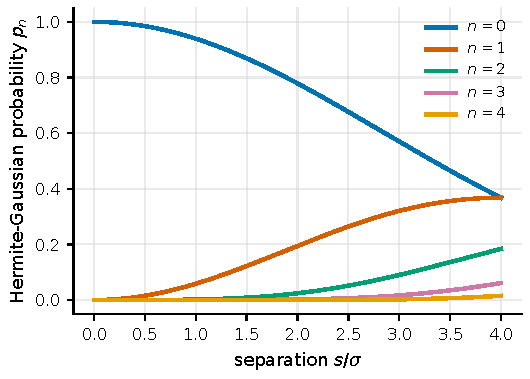
\includegraphics[width=0.82\linewidth]{figures/generated/chapter_08/ch08_spade_probabilities.pdf}
\caption{理想 Hermite--Gauss 模式排序的模式概率。横轴是间距 \(s/\sigma\)，纵轴是每个模式的单光子概率。小间距时 \(p_0\) 仍接近 1，而 \(p_1\) 及更高模式按 \(Q=s^2/(16\sigma^2)\) 的幂次抬头；间距信息正是由这些低概率模式的计数携带。}
\label{fig:e12-spade-prob}
\end{figure}

\begin{figure}[tbp]
\centering
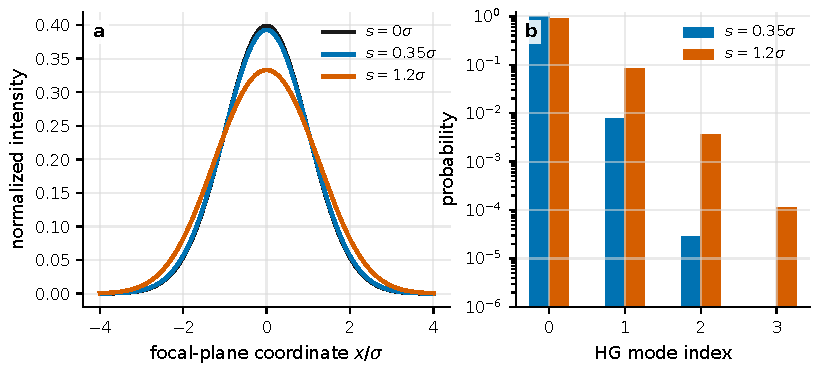
\includegraphics[width=0.92\linewidth]{figures/generated/chapter_08/ch08_direct_image_vs_modes.pdf}
\caption{同一双源模型在直接像面与模式输出中的两副面孔。左：\(s=0\)、\(0.35\sigma\)、\(1.2\sigma\) 的归一化像面强度，亚分辨时曲线差别只是极弱的展宽。右：\(s=0.35\sigma\) 与 \(1.2\sigma\) 时前四个 Hermite--Gauss 模式的概率，低阶非基模概率虽小，却把间距变成了清清楚楚的模式计数。}
\label{fig:e12-direct-vs-modes}
\end{figure}


\section{现实的限制：量子下界不是自动可达}
\label{sec:e12-reality}

漂亮的 \eqref{eq:e12-mode-saturates} 有一个大前提：模式基底精确对准了真实质心，而且模式排序器没有串扰、没有背景漏光。现实里这些都要打折扣，量子下界会被一层\textbf{系统误差平台}（systematic floor）顶住。

最致命的是\textbf{质心/指向误差}（centroid / pointing error）。SPADE 的第一阶模式 \(u_1\) 靠"整幅图相对模式中心的横向不对称"来装信号。可如果整幅图因为指向抖动、跟踪误差而整体偏了 \(\delta x\)，那这偏移\emph{本身}就会往 \(u_1\) 里灌光——而且机制和真信号一模一样。用上一节同样的相干态换算，整体偏移 \(\delta x\) 漏进第一阶模式的比例是
\[
  p_1^{\rm leak}\approx\frac{\delta x^{2}}{4\sigma^{2}},
\]
而真正的双星信号是 \(p_1^{\rm sig}\approx s^2/(16\sigma^2)\)。两者相等的条件是
\[
  \frac{\delta x^{2}}{4\sigma^{2}}=\frac{s^{2}}{16\sigma^{2}}
  \ \Longrightarrow\ \delta x=\frac{s}{2}.
\]
换句话说，只要质心标定误差达到间距的一半，赝信号就和真信号同量级——这时你测到的第一阶计数根本分不清是"两颗星"还是"望远镜没对准"。要测 \(s=0.1\sigma\) 的间距，就得把质心稳定和标定到远好于 \(0.05\sigma\)，这对指向、跟踪和标定是很硬的要求。

除此之外还有一串现实杀手：模式排序器的\textbf{串扰}（crosstalk）矩阵不稳定，会把 \(u_0\) 的强光漏一点到 \(u_1\)，淹没万分之几的信号；\textbf{背景光}若不具有和源相同的空间模式分布，会在各模式里铺一层底噪；Strehl 比不够、像差随时间漂、色散和偏振串扰都会污染模式响应矩阵。这些效应的共同特征是：它们\emph{不随 \(N_\gamma\) 下降}。统计误差按 \(1/\sqrt{N_\gamma}\) 一路降，可一旦撞上系统平台，再加光子也没用（图 \ref{fig:e12-crb} 里那条加了标定误差就压平的绿线，画的正是这件事）。所以"达到量子下界"从来不是自动的，实验上更常见的是较简单、较稳健的相位敏感测量（相位板、SLIVER、SPLICE 一类），它们缓和了直接成像的二次损失，但实际增益仍由可见度、串扰和对准误差说了算 \citep{2017PhRvL.118g0801T,2019NJPh...21i3010B,2018Optic...5.1177P}。

\begin{figure}[tbp]
\centering
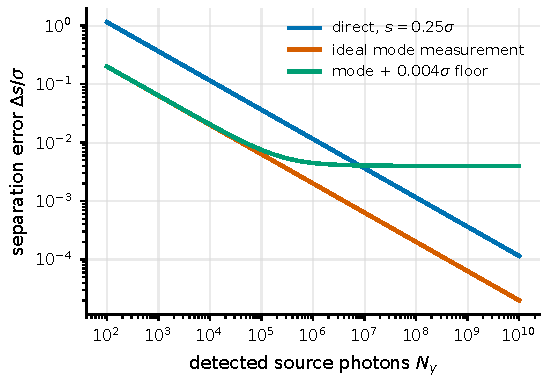
\includegraphics[width=0.82\linewidth]{figures/generated/chapter_08/ch08_cramer_rao_bound.pdf}
\caption{亚分辨双源的 Cramér--Rao 间距误差。横轴是探测源光子数 \(N_\gamma\)，纵轴是 \(\Delta s/\sigma\)。理想模式测量按 \(N_\gamma^{-1/2}\) 一路下降；直接成像因 Fisher 信息小得多，要更多光子才追平。绿线加入一小段模式匹配系统误差后出现平台——继续加光子也消不掉标定误差。}
\label{fig:e12-crb}
\end{figure}

还有一层更微妙的前提：源的\textbf{部分相干}（partial coherence）。上面全程假设两颗星互不相干（等权概率混合）。Larson 与 Saleh 指出，当源变得部分相干时，Rayleigh 诅咒可能\emph{重新出现}；Tsang 与 Nair 随后澄清，只要不是完全正相关的退化情形、并对弱热光做正确的 Fisher 计算，SPADE 仍能避免小间距信息彻底消失 \citep{2018Optic...5.1382L,2019Optic...6..400T}。天文学里尤其要分清两件事：源面上两块辐射区\emph{本身}独立不独立发光，与光传播到望远镜后、由 van Cittert--Zernike 定理（第 \ref{chap:e10} 章）造出的空间相干，是两码事。后者正是干涉测量要测的量，不能简单等同于源本身的相干发射。


\section{长基线的版本：强度干涉在傅里叶平面做同一件事}
\label{sec:e12-sii}

前面几节讲的是单孔径、或相干合束之后的空间模式测量。可"把分辨率当估计问题"这套思路，完全可以搬到公里级长基线阵列上去——只是这次舞台从像面换到\textbf{傅里叶平面}（Fourier plane）。第 \ref{chap:e10}、\ref{chap:e11} 章讲过：不同望远镜对之间的基线，采样天空亮度分布的不同空间频率；数据的约束来自\emph{可见度随基线怎么变}。这里的"亚分辨"，不再是从一个衍射斑里读两个峰，而是在长基线上量出源亮度分布的傅里叶模长。

强度干涉（intensity interferometry）不测一阶场相位，而测两台望远镜光强\emph{涨落}的相关。理想热光下，零延迟的二阶相关（第 \ref{chap:e10} 章的 Siegert/HBT 关系）给出

\begin{equation}
  g_{ij}^{(2)}(0)-1=\big|\gamma_{ij}\big|^{2},
  \label{eq:e12-hbt}
\end{equation}
\begin{formulaexplain}
\(g_{ij}^{(2)}(0)\)：望远镜 \(i,j\) 零时延二阶相关；减 1 得相对于"毫不相关"基线的超出。\(\gamma_{ij}\)：归一化复相干度，等于一阶可见度 \(V\)。强度涨落的同步程度，直接给出可见度模平方。
\end{formulaexplain}

于是观测量是一串基线/谱道/时段上的平方可见度：

\begin{equation}
  d_{k}=\big|V(u_k,v_k;\bm\theta)\big|^{2}+\eta_{k},
  \label{eq:e12-sii-data}
\end{equation}
\begin{formulaexplain}
\(d_k\)：第 \(k\) 个基线/时间/谱道上测到的平方可见度。\(V\)：源参数 \(\bm\theta\) 决定的模型可见度。\(\eta_k\)：噪声。角结构就写在 \(|V|^2\) 随基线的变化里。
\end{formulaexplain}

把同样的 Cramér--Rao 逻辑套上去。对参数 \(\theta_\alpha\)，强度干涉的 Fisher 矩阵是

\begin{equation}
  F_{\alpha\beta}^{\rm SII}
  =\sum_{k,l}
  \frac{\partial|V_k|^{2}}{\partial\theta_\alpha}\,
  C^{-1}_{kl}\,
  \frac{\partial|V_l|^{2}}{\partial\theta_\beta},
  \label{eq:e12-sii-fisher}
\end{equation}
\begin{formulaexplain}
\(F_{\alpha\beta}^{\rm SII}\)：强度干涉数据的 Fisher 矩阵。\(C^{-1}_{kl}\)：\(|V|^2\) 测量误差协方差的逆，给数据点加权。可见度模平方对参数越陡、误差越小，信息越多。
\end{formulaexplain}

其中 \(C_{kl}\) 是 \(|V|^2\) 测量误差的协方差，可用时间移位背景、空基线、隔夜重复观测或注入模拟来估。若各数据点误差近似独立，\(C\) 变对角，\eqref{eq:e12-sii-fisher} 就退化成"每点斜率平方除以方差再求和"——和单参数 \eqref{eq:e12-fisher-def} 是同一件事，只是求和取代了积分。要害在那个\emph{斜率} \(\partial|V|^2/\partial\theta\)：它告诉你哪条基线最有用。

代一个具体模型——均匀圆盘恒星。它的可见度是一阶 Bessel 函数（这来自圆盘亮度分布的傅里叶变换，第 \ref{chap:e10} 章推过）：

\begin{equation}
  V(x)=\frac{2J_1(x)}{x},
  \qquad x=\frac{\pi B\theta_\star}{\lambda},
  \label{eq:e12-uniform-disk}
\end{equation}
\begin{formulaexplain}
\(V(x)\)：均匀圆盘的可见度。\(J_1\)：一阶 Bessel 函数。\(B\)：投影基线（米）。\(\theta_\star\)：恒星角直径。基线通过无量纲的 \(x\) 扫描圆盘的傅里叶模长。
\end{formulaexplain}

\(V(x)\) 在 \(x=0\) 处为 1，随 \(x\) 增大先降到第一个零点（\(J_1\) 的第一个非平凡零点在 \(x\approx3.83\)，这是标准的 Bessel 零点），再翻出一串越来越弱的旁瓣。对角直径 \(\theta_\star\) 最有用的基线，落在 \(|V|^2\) 斜率 \(\partial|V|^2/\partial\theta_\star\) 最大的地方——通常在可见度快速下坠的那一段。短基线上 \(V\approx1\)、几乎不随 \(\theta_\star\) 变（平台上没斜率、没信息）；极长基线上信号又掉进旁瓣、容易被系统误差压住。所以"基线不是越长越好"，而是要\emph{挑在斜率大处}。图 \ref{fig:e12-sii-fisher} 把这条设计原则画得很直白。

\begin{figure}[tbp]
\centering
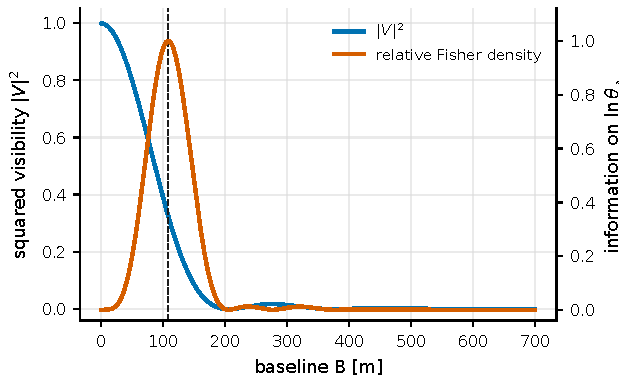
\includegraphics[width=0.82\linewidth]{figures/generated/chapter_08/ch08_visibility_fisher_design.pdf}
\caption{强度干涉里基线选择与参数信息的关系。蓝线是 \(\lambda=450~\mathrm{nm}\)、\(\theta_\star=0.55~\mathrm{mas}\) 均匀圆盘的平方可见度；橙线是按 \(\partial|V|^2/\partial\ln\theta_\star\) 算出并归一化的 Fisher 权重。最有用的基线落在可见度快速下降处；单纯拉长或缩短基线都不会自动增加角直径信息。}
\label{fig:e12-sii-fisher}
\end{figure}

强度干涉的代价是\textbf{相位缺失}：\(|V|^2\) 丢掉了 \(V\) 的相位，因此对整体平移不敏感，还会带来镜像与中心对称退化——二元星的取向、亮斑位置、非对称盘面往往要靠地球自转带来的 \(uv\) 覆盖、多波长、先验模型或三阶相关来缓解。它换来的好处极大：对大气相位扰动几乎免疫。因为它只比较两路\emph{强度}抖动同不同步，望远镜之间只需电子连接、把信号在时间上对齐到探测响应的一小部分即可，不必维持光学相干（第 \ref{chap:e10} 章算过，纳秒级电子时间对应几十厘米的光程容差，大气 piston 那点纳米级抖动完全落在容差里）。正因如此，那些光学像质远不及专业干涉仪、却坐拥大收集面积和长基线的大气 Cherenkov 望远镜阵列，反而成了理想的强度干涉阵 \citep{1956Natur.177...27B,1974MNRAS.167..121H,2020NatAs...4.1164A,2024MNRAS.529.4387A}。

\paragraph{两条工程路线的分工}
\label{sec:e12-two-roads}

把两种"亚分辨估计"并排看，它们的工程瓶颈正好相反，因此适用对象也不同：

\begin{itemize}
  \item \textbf{SPADE / 空间模式测量}（单孔径或相干合束）：要求\emph{稳定的波前}。目标光要耦进光纤模式、集成光学芯片或自由空间模式排序器，自适应光学把入射光尽量压进少数可控模式。它的敌人是 Strehl 比、非共路像差、质心抖动和模式串扰。适合读出两颗近星的角间距、恒星的低阶形状矩这类少参数问题。
  \item \textbf{强度干涉}（长基线阵列）：干脆\emph{接受}大气把相位随机化，用大收集面积和长基线去换 \(|V|^2\) 信息。它的敌人是光子率低、电子带宽、背景、时间同步和系统协方差。适合亮热星、快速自转星、双星和角直径测量。
\end{itemize}

无论走哪条路，一套能拿出去发表的亚分辨估计，都得同时交代四本账：\emph{光子预算}（星等、谱带、总效率、曝光 \(\to\) 有效 \(N_\gamma\)）、\emph{角尺度}（\(\lambda/D\)、PSF 宽 \(\sigma_\theta\)、候选间距 \(s\) 或角直径 \(\theta_\star\)）、\emph{测量矩阵}（像素响应、模式串扰、或 \(|V|^2\) 协方差）、\emph{模型边界与误差拆分}（等亮双源、未知亮度比、有限圆盘、部分相干、背景星怎样改写 Fisher 矩阵）。最后检查一条判据就够诊断：统计误差还在按 \(N_\gamma^{-1/2}\) 下降吗？若不再降，八成是对准、PSF、背景、相关器或模型误差撞上了平台。把这些边界放进最终推断，常用贝叶斯采样与证据比较——直接成像、模式计数、强度干涉数据可以共享同一个参数向量、联合似然相乘；已知轨道、颜色、光谱型、距离等先验会直接改变可识别的参数空间 \citep{2009MNRAS.398.1601F,2013PASP..125..306F}。


\section{本章要点}
\label{sec:e12-summary}

\begin{itemize}
  \item \textbf{分辨率是估计问题，不是成像判据。} Rayleigh 判据 \(\theta_{\rm R}=1.22\lambda/D\) 只问"像面能不能分成两峰"；真正该问的是"给定 \(N_\gamma\) 个光子，间距 \(s\) 能估到多准"，答案由 Fisher 信息与 Cramér--Rao 下界 \(\mathrm{Var}(\hat s)\ge1/F_{ss}\) 给出。
  \item \textbf{小间距先变胖、不先分家。} 把两个平移 PSF 泰勒展开，一阶项相消，\(p(x\mid s)=h+\tfrac{s^2}{8}h''+\mathcal O(s^4)\)。间距最低阶通过 \(h''\) 表现为二阶展宽，直接成像 Fisher 信息 \(F_{ss}^{\rm direct}\simeq N_\gamma s^2/(8\sigma^4)\to0\)——这就是 Rayleigh 诅咒。
  \item \textbf{信息没离开光。} 量子 Fisher 信息把"逐像素"换成"所有允许测量"，对弱热光单光子态得 \(F_{ss}^{Q}=N_\gamma/(4\sigma^2)\)，\(s\to0\) 时不消失。诅咒是测量方式的病，不是光的病。
  \item \textbf{SPADE 饱和量子极限。} 先投到 Hermite--Gauss 模式再计数，模式概率是 Poisson 分布 \(p_n=e^{-Q}Q^n/n!\)，\(Q=s^2/(16\sigma^2)\)。第一阶模式里 \(p_1\propto s^2\)、\(\partial p_1/\partial s\propto s\)，二者在 Fisher 信息中相除留下有限极限 \(N_\gamma/(4\sigma^2)\)，绕开诅咒。
  \item \textbf{下界不是自动可达。} 质心误差 \(\delta x\) 漏进第一阶模式的量 \(\delta x^2/(4\sigma^2)\)，当 \(\delta x\sim s/2\) 时就与信号 \(s^2/(16\sigma^2)\) 同量级；串扰、背景模式、部分相干都会制造不随 \(N_\gamma\) 下降的系统平台。
  \item \textbf{长基线是同一件事的傅里叶版。} 强度干涉在傅里叶平面估参数，\(F^{\rm SII}_{\alpha\beta}=\sum\partial|V|^2/\partial\theta\,C^{-1}\,\partial|V|^2/\partial\theta\)，最有用的基线在 \(|V|^2\) 斜率大处。它丢相位、免大气，与 SPADE 的"稳波前"路线互补。
\end{itemize}

\medskip
\noindent\textbf{想一想。}
\begin{enumerate}
  \item 若把两颗星的\emph{亮度比}也设为未知参数，第一阶（奇）模式和基模（偶模式）各自还剩多少间距信息？为什么"未知亮度比"这个退化，会削弱奇模式的贡献？
  \item 直接成像的 \(F_{ss}^{\rm direct}\propto s^2\) 是在\emph{高斯} PSF 下推的。换成有真实旁瓣的 Airy PSF，二阶展宽这一步会不会改变？Rayleigh 诅咒是高斯的特产，还是更普遍的现象？
  \item 强度干涉丢掉了相位，SPADE 保留了模式的相对相位信息。对"测两颗近星的\emph{取向}"这个任务，哪一种更有优势？把它翻译成 \eqref{eq:e12-sii-fisher} 里的退化来说明。
\end{enumerate}
